\section{Literature review}
\label{sec:litreview}
The following literature review gives an overview of existing deployable booms developed, computer simulations used to model these booms and an explanation of moment rotation curves. 
\subsection{Examples of deployable structures}
% trac boom 
%STEM
\begin{wrapfigure}{l}{0.5\textwidth}
  \begin{center}
     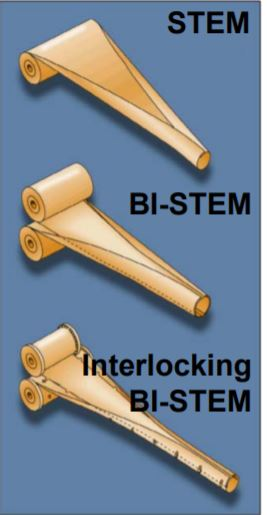
\includegraphics[width=0.3\textwidth]{images/stemderivatives.JPG}
  \end{center}
  \caption{STEM boom and its derivatives image obtained from source \cite{NorthropGrumman}}
  \label{fig:boom}
\end{wrapfigure}
The first type of deployable structure used in space was the Astro Aerospace Storable Extendible Tubular Member (STEM) \cite{NorthropGrumman}. Flown since the 1960's it has proven flight heritage which includes applications on the Voyager spacecraft and the Apollo missions to the moon \cite{NorthropGrumman}. The STEM is a boom with a curved cross section shown in figure \ref{fig:boom}. It rolls up flat on a drum returns to its circular shape after deployment\cite{NorthropGrumman}. The stowed STEM fits into a small space and can be used to deploy/retract other structures like Antennas, Telescopes, Solar array support structure etc. The STEM booms have a simple mechanism and is lightweight. However it has low torsional stiffness and has the tendency to buckle under compression. 
%BI-STEM
A derivative was created to make the booms torsionally stiffer called the BI-STEM booms also shown in figure \ref{fig:boom}. This design includes the use of two STEM booms, one over the other. Because of a closed circular section this type has a higher torsional stiffness which makes it less susceptible to buckling under compression. Further when the STEM booms are being deployed they cause dynamic instabilities in the spacecraft. A BI-STEM boom solves this problem as the two boom motors effectively counter torque each other to provide dynamic damping\cite{Thomson2018}. However this design needs a bigger volume to stow. The loading capability and buckling resistance is limited by the packaging restrictions of these type of booms. Novel methods such as in-orbit bonding of BI-STEM booms are proposed by Schmidt et. al.\cite{Tilo}. 
%CTM
The Collapsible tube mast (CTM) boom \cite{dlr} consists of two laminated sheets which are bonded at the edges to form a tubular shape as shown in figure \ref{fig:ctm}. In the deployment phase the boom is flattened and coiled up on a central hub for storage. During the deployment phase, once the booms are uncoiled they reach their full stiffness by enlarging to its original circular shape. The cross sectional shape gives the boom additional bending stiffness which overcomes the shortcoming of the open cross section of the STEM booms \cite{Fernandez2017}. Thus for the same deployed diameter, the CTM boom has half the packaged height as the STEM and requires less strain to flatten \cite{Murphey2011}. However due to prolonged stowage, significant cross section flattening was observed \cite{Fernandez2017} which reduced the load bearing capacity by 50\%. 
\par
%tapespring
More recently, developed for the deployable mechanisms of satellite de-orbiter, CopperBeryllium (CuBe) tape springs offer an alternate solution \cite{Fernandez2013}, which look like STEM booms shown in figure \ref{fig:boom}. Two CuBe springs face each other to form a lenticular cross-section. The two tape springs are then encased by a Kapton sheath to form a closed cross-section with an improved torsional stiffness and buckling load. As the booms are coiled for storage, the two tape springs will slide with respect to each other inside the Kapton sheath, thereby reducing the amount of shear stress and strain energy stored in the stowed configuration. \cite{Fernandez2013}
%BRC
The Rolatube used in Inflatsail satellite in 2017\cite{Rolatube} in an example of bistable reeled composites which are stable in both deployable and stowed configuration due to their composite laminate design. Due to this property, these type of booms dont require a restraining device, however it is often in practice that satellites carry a motor to deploy these booms in order to control the deployment of the booms. 
%multiangle braids
Carbon fibre booms in a coiled state experience high strains which can cause delamination and creep effects on the material \cite{Fernandez2013}. The Open section CFRP booms utilise an interesting innovation to reduce the high strain during the stowed configuration. By varying the braid angle quasi-linearly from root to tip (respectively 50\degree and 35\degree), the natural coiling radius will vary linearly along the boom length, and the boom will thus coil into an Archimedean spiral \cite{Fernandez2013}. This ensures that the four co-coiled booms will be in their lowest energy state possible and in a stable configuration, and no edge buckling will take place. Creep effects during long term storage are also reduced with this approach. 
%shearless
\par
\begin{wrapfigure}{r}{0.5\textwidth}
  \begin{center}
     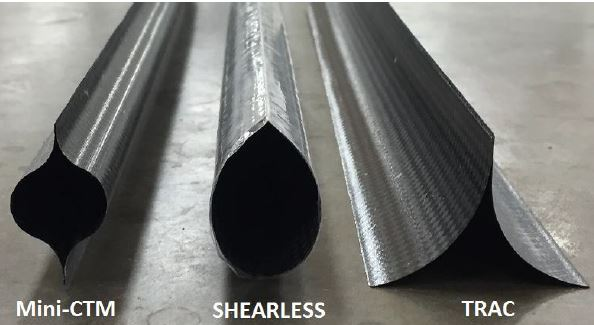
\includegraphics[width=0.48\textwidth]{images/ctmshearless.JPG}
  \end{center}
  \caption{CTM, SHEARLess and TRAC booms \cite{Fernandez2017}}
  \label{fig:ctm}
\end{wrapfigure}
SHEAth-based Rollable LEnticular-Shaped and low-Stiction (SHEARLESS) boom \cite{shear} is fabricated from joining two independent tape-springs front-to-front with the use of a durable seamless polymer sleeve. This sleeve allows the two parts to slide past each other during the coiling/deployment process so as to minimize shear and its derived problems. And during storing of the boom, it first flattens and then the two tape springs axially slide against the polymer. Thus the shear stresses are endured by the flexible sheath rather than the bond line. The main advantage of this design is that it reduces tendency of the inner shell undergoing compression to buckle locally giving an improvement over the TRAC and CTM booms with little increase in mass or complexity \cite{Fernandez2017}. The sheath encloses and couples the two inner shells so there are no problematic adhesive bonds in the design and long term stowage creep effects are thus reduced. As in CTM designs, the doubly-symmetrical cross-section of the SHEARLESS boom makes the centroid (neutral axis) and the shear center coincident. This eliminates undesired flexural-torsional coupling that can often cause buckling and collapse in torsionally weak slender booms like these.\cite{Fernandez2017} However the current challenge is computational modelling of the SHEARLESS booms as they give largely non linear responses.\cite{Fernandez2017}
%TRAC 
\par
The US Air Force Research Laboratory developed the Triangular Rollable and Collapsible (TRAC)  boom shown in figure \ref{fig:boom}. This boom is made of two curved C-shaped sections joined along one edge \cite{Murphey2011}. This results in a large cross-section inertia to packaged height ratio compared to STEM and CTM architectures \cite{Murphey2011}. Even though this design reduces the torsional stiffness of the boom, bending stiffness is the limiting measure of performance for most applications\cite{Murphey2011}. In addition, the strain required to flatten the flanges of a TRAC boom are smaller than the STEM or the CTM booms allowing for thicker flange materials to be used \cite{Murphey2011}. This results in greater bending stiffness as compared to the aforementioned boom types. Predicted performance of the TRAC boom indicate 10 times greater bending stiffness than a CTM boom with the same packaged height and material and 34 times greater bending stiffness than a STEM boom \cite{Murphey2011}.
%Bi-TRAC
\par
TRAC booms which are bi-stable in both deployed and stowed configurations are called Bi-TRAC booms. The inner shell of the beam is made with a Bi-stable laminate and the outer shell is made with a less stiff laminate with a larger strain to failure capacity. The main advantage of the bi-TRAC boom is its more predictable and controlled deployment dynamics from coiled to deployed state. For example, a 0.3m Bi-TRAC boom can take 6-8s to self deploy compared to tenths of seconds a TRAC boom would take. Thus it would be a lighter and less complex mechanism.

In summary the following deployable booms have been discussed as given in the table below.  
\begin{table}[!hbt]
\centering
\begin{tabular}{|l|l|}
\hline
\textbf{\begin{tabular}[c]{@{}l@{}}Deployable boom type\end{tabular}} & \textbf{Key features} \\ \hline
STEM & \begin{tabular}[c]{@{}l@{}}Deployable, lightweight, small\\ Low torsional stiffness \\ Low buckling stiffness\end{tabular} \\ \hline
Bi-STEM & \begin{tabular}[c]{@{}l@{}}Higher torsional stiffness\\ Counter torque when deployed\\ More volume to stow\\ Non interlocked tapes\end{tabular} \\ \hline
CTM & \begin{tabular}[c]{@{}l@{}}Half the packaged height\\ Requires less strain to fold\\ Flattening of boom causes less load bearing capacity\end{tabular} \\ \hline
TRAC & \begin{tabular}[c]{@{}l@{}}Higher bending stiffness \\ Strain required is lesser\end{tabular} \\ \hline
Bi-TRAC & More stable when self deploying \\ \hline
SHEARLess & \begin{tabular}[c]{@{}l@{}}Higher buckling resistance\\ 2 tape booms are enclosed by a sheath\end{tabular} \\ \hline
\end{tabular}
\caption{Summary of deployable structures}
\end{table}
\begin{comment}
Oxford space systems have developed ASTROTUBE\texttrademark \hspace{0.1 cm} BOOM which supports a wide range of Microsat and cubesat application \cite{Oxfordspacesystems}.They have also been flight proven on the AlSat-Nano3U cubesat \cite{Oxfordspacesystems}. The boom element can be fully or partially deployed which is a result of a greater control of the deployment sequence as compared to the rollable booms. \cite{EoPortal}.
\end{comment}
\subsection{Computational modelling}
A computational modelling approach is selected in this report in order to study the effects of boundary conditions to better model conditions found in space, where the booms are meant to operate in. An overview of the computational models of STEM booms are given. These techniques are later used in the model developed for this paper. 
%boundary conditions etc. 
%BRC
Dynamic analysis of a cantilevered boom BRC attached to solar sails was conducted in FE package ABAQUS by Wu et. al \cite{Wu2018}. The Budiansky Hutchinson criteria\cite{Budiansky} was used to find the instability criteria based on changes in cross section. It was found that the buckling occurs at different accelerations for same sense bending and opposite sense bending, with the same sense bending occurring faster. The spacecraft was assumed to be a rigid square plate to which an extended Bistable reeled composite (BRC) is attached. 
One end of the BRC boom is tied rigidly to the square plate using a 'Master Slave' algorithm in ABAQUS. For the loads modelling an angular acceleration is used. S4R shell elements with reduced integration to model the composite booms as they are robust and have a lower computational cost. 
The Budiansky-Hutchinson criterion \cite{Budiansky} for shell structures which states that dynamic stability loss occurs when the maximum deflection grows rapidly with the small variation of the load amplitude is used to estimate the critical angular acceleration that booms can sustain before becoming unstable during a spacecraft's rotational manoeuvre. 
The cross-section deformation in the transverse direction, $\xi$ is used as the key parameter to estimate the maximum angular acceleration. To validate the experiment, the behaviour of a boom in microgravity is extremely difficult however it is possible to simulate the g value in linear acceleration.
A laser distance gauge was used to measure the end displacement of the boom. A correlation with an approx 5.9\% difference was found between the experimental and simulated tip displacement. 
This result was used to verify the bending reliability of the FE simulation. Using the Budiansky-Hutchinson criterion the critical rotational acceleration can be found for the single boom and validated against the FE results. However in this paper it is assumed that the base of the boom connected to the satellite would have all 6 degrees of freedom constrained with no change in geometry \cite{Wu2016}. This end condition is not representative of the satellite deployer attachment and can give inaccurate results.
\subsection{Moment rotation curve}
\begin{figure}[!hbt]
    \centering
     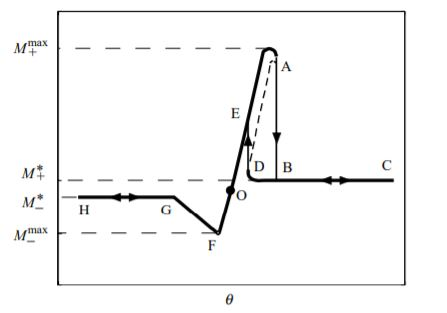
\includegraphics[width=10cm]{images/tapespring.JPG}
     \caption{Tape spring reaction moment vs rotation curve \cite{Seffen1999}}
  \label{fig:tapetheory}
\end{figure}
Tape springs have the same moment vs rotation curve as that of the STEM booms. The non-linear behaviour exhibited by them are studied in this overview which are used to explain the results obtained in section \ref{sec:results}. 
The figure \ref{fig:tapetheory} shows the relationship between the reaction moment and the rotational moment of a tape spring where point O is the neutral point where no displacement is applied. A positive moment in this case is referring to opposite sense bending and a negative moment is referring to same sense bending shown in figures \ref{fig:same} and \ref{fig:opp}. 
As the same sense bending moment is applied to the tape spring, the curve linearly progresses to the point F after which it snaps and the propogating moment stays constant for increase in $\theta$. If a negative moment is applied, the linear behaviour ends much sooner. At point F there is a sudden snap that results in a flexural-torsional deformation mode with a formation of a fold \cite{Seffen1999}.
From this point onwards M remains constant as $\theta$ is further increased (points G to H) \cite{Seffen1999}. When $\theta$ is decreased, the unloading path practically coincides with the loading path \cite{Seffen1999}. It can be seen that the peak moment for same sense bending is lesser than the peak bending moment of the opposite sense bending because the flexural-torsional mode of failure in the same sense bending occurs sooner than the buckling mode of failure in the opposite sense bending \cite{Seffen1999}. 
In reference \cite{Seffen1999}, it is mentioned that an elastic fold developed that is sufficiently far away from the ends of a tape spring consists of two symmetric transition regions on either side of a cylindrical region with uniform curvature \cite{Seffen1999}. The angle subtended by this cylindrical region is approximately equal to the relative rotation $\theta$ between the ends of the tape spring, as both the transition regions and the remaining parts of the tape spring have negligibly small longitudinal curvature \cite{Seffen1999}.
It has been shown that in the absence of end effects the bending moment at the fold remains approximately constant as $\theta$ varies \cite{Seffen1999}. 
This behaviour changes when the fold reaches near the built-in end, where the cross-sectional shape is held rigidly fixed. Here the fold stops moving but only $\theta$ can change. 
